\chapter{Introduction}

In recent years, the field of giant planet formation has aimed to answer two fundamental questions:

\begin{enumerate}
\item Where in the protoplanetary disk can gas giants form?
\item What compositions will the formed giant planets have obtained?
\end{enumerate} 

We can start uncovering the answers to these questions through a combination of studying planet formation in protoplanetary disks, the end-results of planet formation (i.e., exoplanets), and through comparisons with the architecture and composition of our own Solar System. Within the last two decades, more than one thousand extrasolar planets (exoplanets)
have been discovered \citet{batalha14}. Their diversity in terms of mass, radius, location and composition
\citet{lissauer14} provides an exciting field of research, with the eventual goal of finding planets that are
similar to our own Earth and may sustain life. For this purpose, it is thus crucial to explore
and understand how planets obtain their compositions. Observations of Earth-like planets
that can provide useful insight about their composition are challenging --- the solid interior
structure of terrestrial planets cannot be detected, and their gaseous envelopes are small by
comparison (both in mass and radius), which makes it difficult to obtain atmospheric spectra
and find out what chemical compounds they are made of. We therefore turn to giant planets,
which have provided a rich and intriguing research area for decades. Gas giants contain most
of their mass in their atmosphere, hence their chemical composition is determined by that
of their envelopes. The last few years have seen a substantial increase in the number of
giant planets with observed atmospheric spectra (e.g., \citealt{debes13}, \citealt{kreidberg15}), which has enhanced our
understanding of these planets� chemical structure, and has provided us with quantitative
information about the abundances of various compounds in their envelopes besides hydrogen
and helium. Finally, gas giants shape the architecture of planetary systems and affect the
delivery of volatile compunds to terrestrial planets, which has direct consequences for the
habitability of worlds similar to our own. Thus testing theories of planet formation against
gas giant compositions will help constrain planet formation theories more generally.


Both terrestrial and giant planets are born in protoplanetary disks, which implies that
their compositions are determined by and tightly linked to the structure and
composition of the disk. The chemical and dynamical evolution of disks, as well the
formation of giant planets have both been previously investigated in isolation. However, the
coupled chemo-dynamical disk evolution, planet compositions, and most importantly the
disk-planet connection have not yet been considered in detail. In this thesis, we uncover some of the answers to this issue from two standpoints: (1) by looking at the role of disk location in setting the conditions for the formation of wide-separation gas giants, and (2) by investigating how the structure and chemical composition of the protoplanetary disk at different radii affects the composition of nascent giant planets.




\section{Dynamics and Chemistry in Protoplanetary Disks}

Protoplanetary disks are the result of the collapse of a molecular cloud, and are structures composed of gas and dust that are rotationally supported and that represent the birth environment of planets (Figure \ref{fig:proto}). Disks are complex objects, whose structure and evolution are affected by a multitude of chemical and dynamical processes. The latter include transport of both dust through radial drift and gas through viscous gas accretion, as well as grain growth and dust settling to the disk midplane, which affect the disk structure. In terms of chemistry, the strongly irradiated disk surface is dominated by photochemical reactions, while the ionized lower layers have a rich ion-molecule chemistry. Finally, the cold disk midplane is mostly shielded from irradiation, and volatile compounds experience freeze-out.  Many of these processes are summarized in \citet{henning13}, and several of them are not yet fully understood.  Moreover, the timescales for various disk chemical and dynamical processes may be comparable at least in some parts of the disk \citep{semenov11}, which makes the coupling between chemistry and dynamics very challenging. As a first step it is thus easier to isolate the different dynamical and chemical processes that occur in the disk midplane where planets are born, and understand their role and relative importance in shaping disk and planet compositions. We explore some of these processes in Chapters 4 and 5, and investigate their consequences for the compositions of giant planets forming at different radii. 

\begin{figure}[h]
\centering
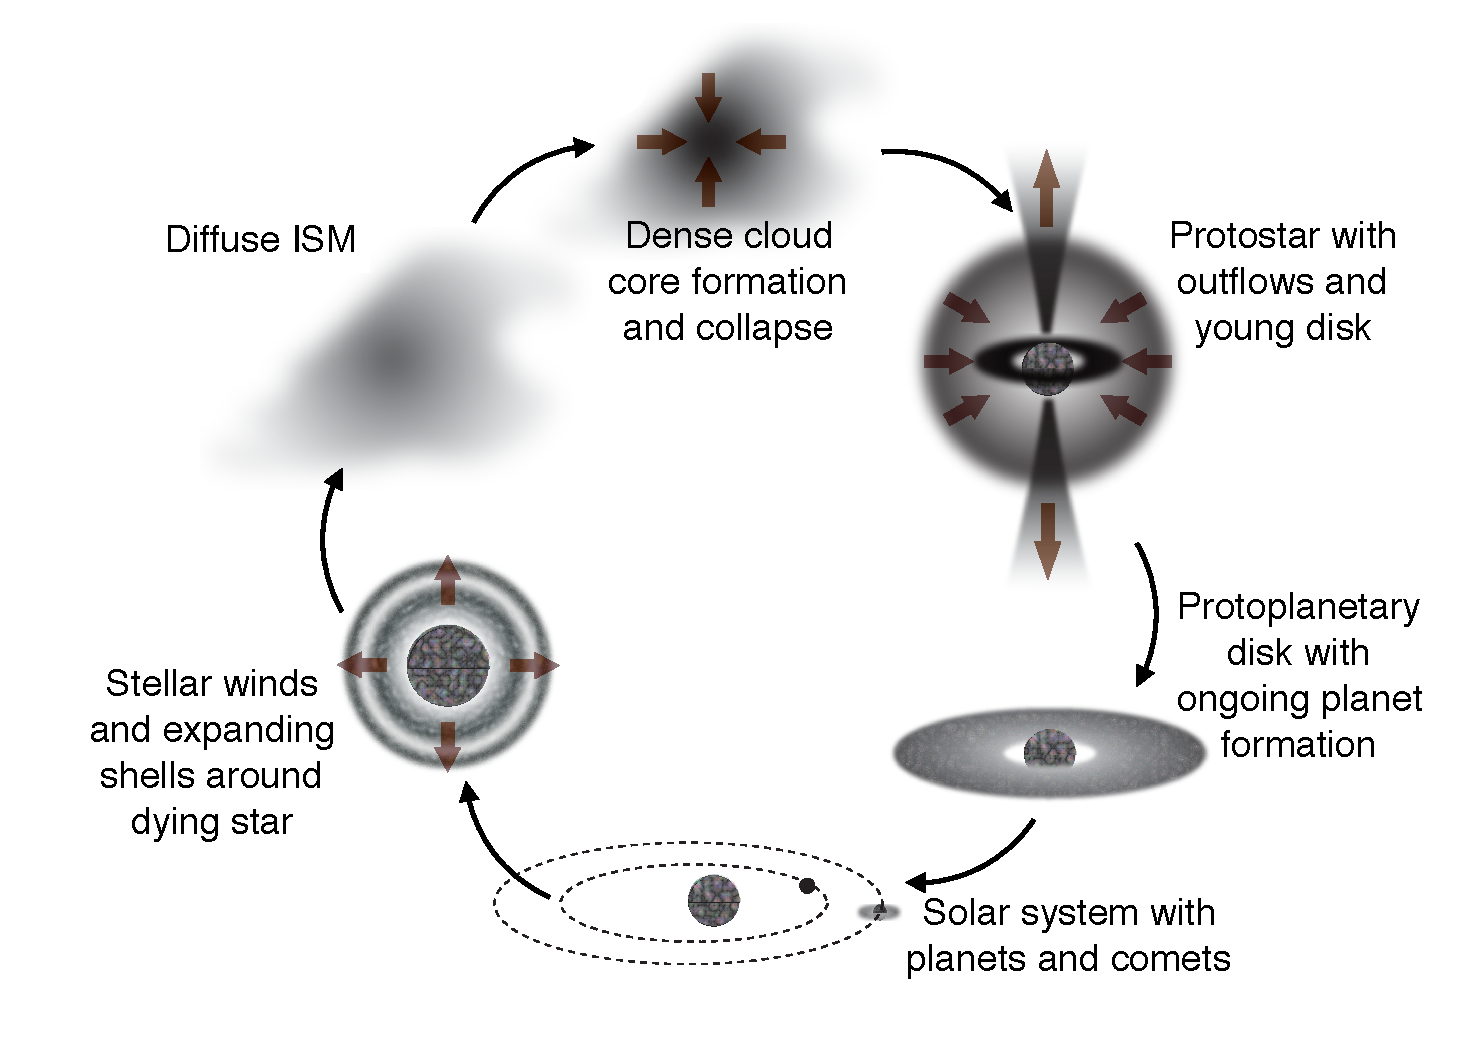
\includegraphics[width=0.8\textwidth]{figures/proto.pdf}
%\vspace{-0.5in}
\caption{The standard picture of molecular cloud to protostar to protoplanetary disk to planet formation. Reprinted by permission from Karin \"Oberg.}
\label{fig:proto}
\end{figure}

%\subsection{Disk Temperature and Density Structure}
\subsection{Disk Temperature and Density Structure}

The midplane temperature in a protoplanetary disk is set both by the irradiation from the host star and by accretion heating (e.g., \citealt{armitage10}). Accretion heating dominates in the inner disk (typically within a few AU) where the accretion flows are strongest, while the outer disk is dominated by stellar irradiation. While the irradiation component of the temperature simply follows a power-law in radius, the accretional component is determined by viscosity and the gas mass accretion rate, which in turn depend on the temperature itself, as well as the gas surface density (for a more complete review see \citealt{shakura73}). As the gas surface density changes with time in an active disk, it follows that determining the midplane temperature in an active disk in which both stellar irradiation and accretion heating contribute to the thermal evolution of the disk is non-trivial. We simplify this problem in Chapters 4 and 5 by assuming a steady-state disk with a constant mass accretion flow, and by solving the thin disk Shakura-Sunyaev equations.

The gas surface density in a viscous disk follows the continuity equation, and is set by both the disk temperature and viscosity. Infall of material onto the disk or outflow may also contribute to the gas surface density evolution \citep{birnstiel10}. The dust surface density can be described by an advection-diffusion equation (e.g., \citealt{birnstiel12}), where both the radial movement of the dust and diffusion contribute to its evolution. The diffusion term is due to the fact that the dust is turbulently mixed by the gas, which causes a change in the dust-to-gas ratio and thus a radial gradient in the ratio between solid and gas surface densities. In the case of small particles that are well coupled to the gas, the surface density follows that of the gas and a constant dust-to-gas ratio is maintained. The movement of larger particles, however, is affected both by radial drift, gas drag and diffusion, which cause the dust surface density to "decouple" from that of the gas. This results in depletion of solids in some disk regions and a pile-up in others, depending on a particle's radial drift velocity and the level of turbulent mixing. The dust surface density is further affected by grain growth and fragmentation. We do not address all these effects in Chapter 4 and 5, and instead assume a constant inflow of particles such that the dust surface density remains spatially and temporally constant. We note, however, that these effects have to be taken into account for a more realistic modeling of the dust surface density, and thus of the surface density evolution of volatiles, both in solid and gaseous form.  





%\begin{figure}[t!]
%\centering
%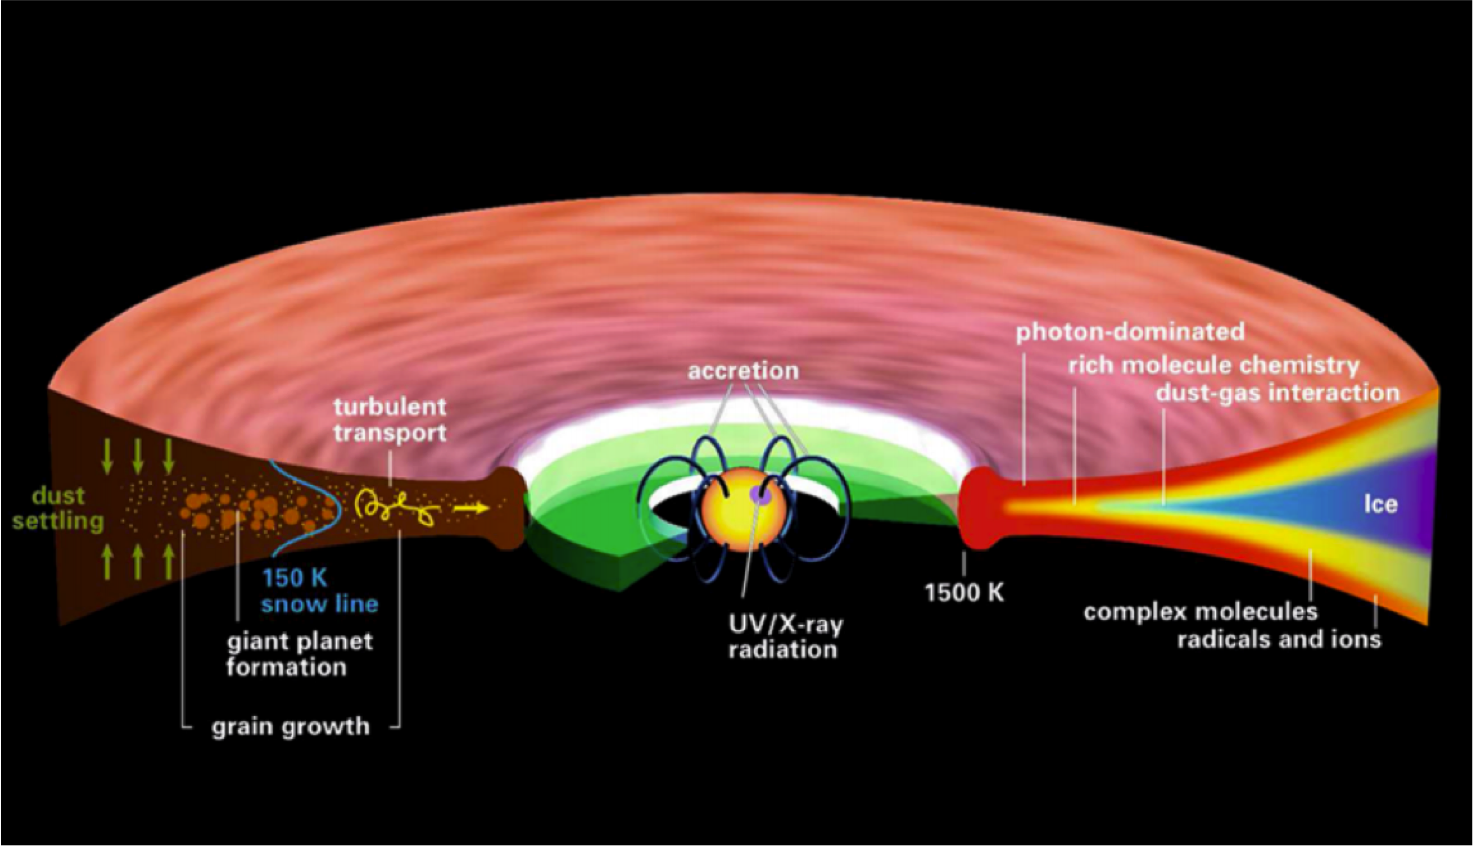
\includegraphics[width=0.8\textwidth]{figures/disk.png}
%%\vspace{-0.5in}
%\caption{Cross section through a protoplanetary disk showing various chemical and dynamical processes that occur in disks. From \citet{henning13}.}
%\label{fig:disk_henning}
%\end{figure}

%\begin{figure*}[t!]
%\centering
%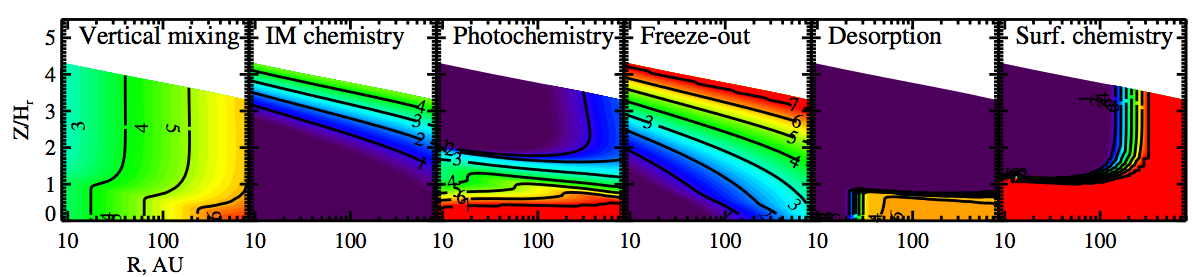
\includegraphics[width=0.8\textwidth]{figures/chemical_timescales.png}
%%\vspace{-0.5in}
%\caption{The distribution of characteristic chemical and dynamical timescales $\tau$ in disks as a function of semi-major axis and height. The numbered curves are $\log_{10} (\tau)$ in million years. From \citet{semenov11}}
%\label{fig:timescales_semenov}
%\end{figure*}

\subsection{Snowlines and Disk Dynamics}

Volatile compounds, which have low sublimation temperatures, are of particular importance. Their relative abundance in gaseous and solid form determines their snowline location, i.e. the distance in the disk where a volatile transitions from gaseous to solid form.  Snowlines are essential in the planet formation process (e.g., \citealt{pontoppidan14}): they can enhance the amount of solid material just outside the snowline, due to dust sublimation, and they can produce pressure traps where dust particles pile up just inside the snowline. Observational advancements in recent year have provided us with an increasing amount of information regarding volatiles in disks. Volatile compounds have been detected in disks (e.g., \citealt{henning13}), which gives us clues about their abundance in different disks and at different disk locations. Moreover, with the advent of ALMA volatile snowlines have also been observed. This is essential as it provides us with knowledge regarding volatile abundances in gas and dust throughout the disk, and thus the compositions of giant planets. Figure \ref{fig:qi13} shows the detection of the CO snowline in TW Hya at 30 AU \citep{qi13}. This snowline has been detected indirectly through its tracer molecule N$_2$H$^+$, which becomes highly abundant as CO freezes out. Moreover, the H$_2$O snowline has also been detected in Tw Hya \citep{zhang13}, as well as the CO snowline in HD 163296 \citep{qi15}. 

%\begin{figure}[t!]
%\centering
%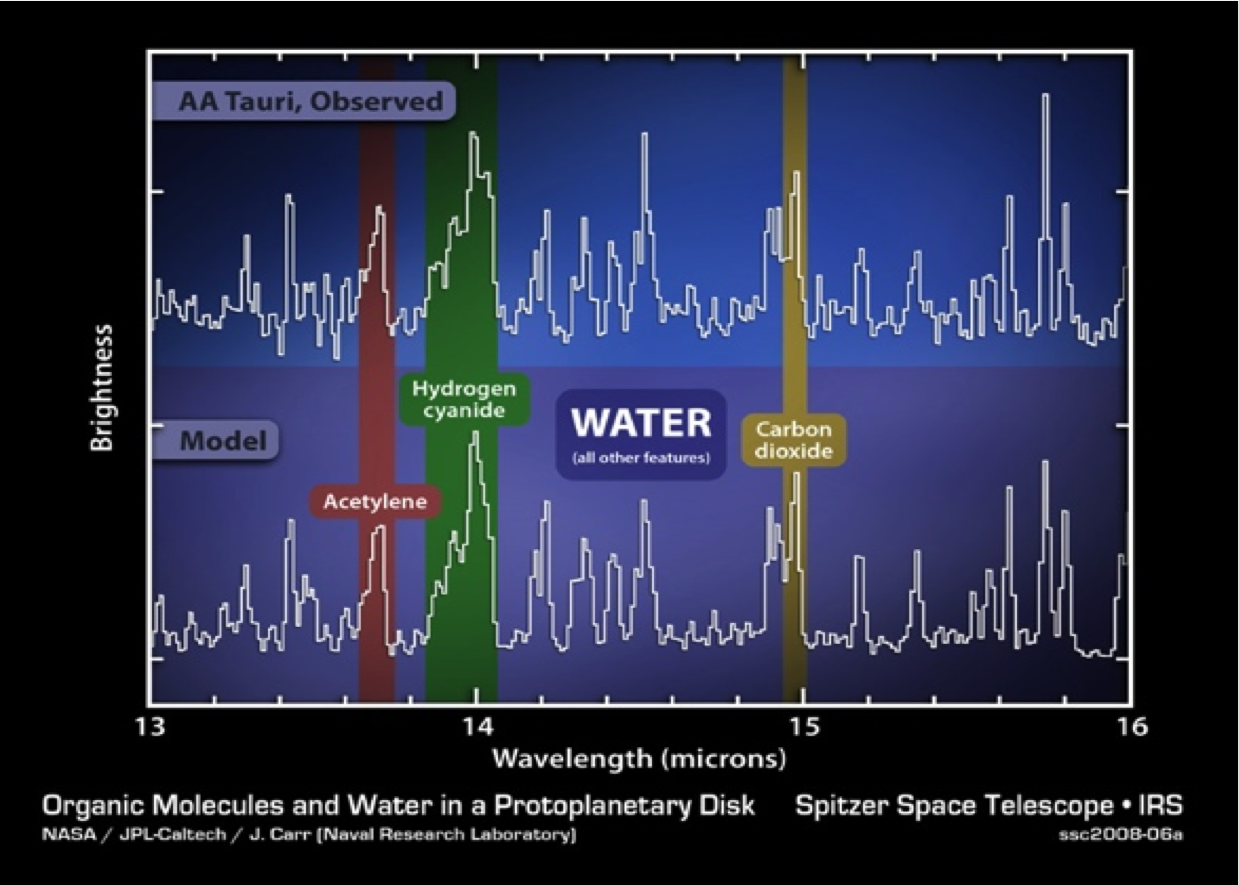
\includegraphics[width=0.8\textwidth]{figures/spitzer.png}
%%\vspace{-0.5in}
%\caption{Spitzer IR spectrum of the disk around AA Tauri showing detections of acetylene, hydrogen cyanide, carbon dioxide and water.}
%\label{fig:spitzer}
%\end{figure}

\begin{figure}[h]
\centering
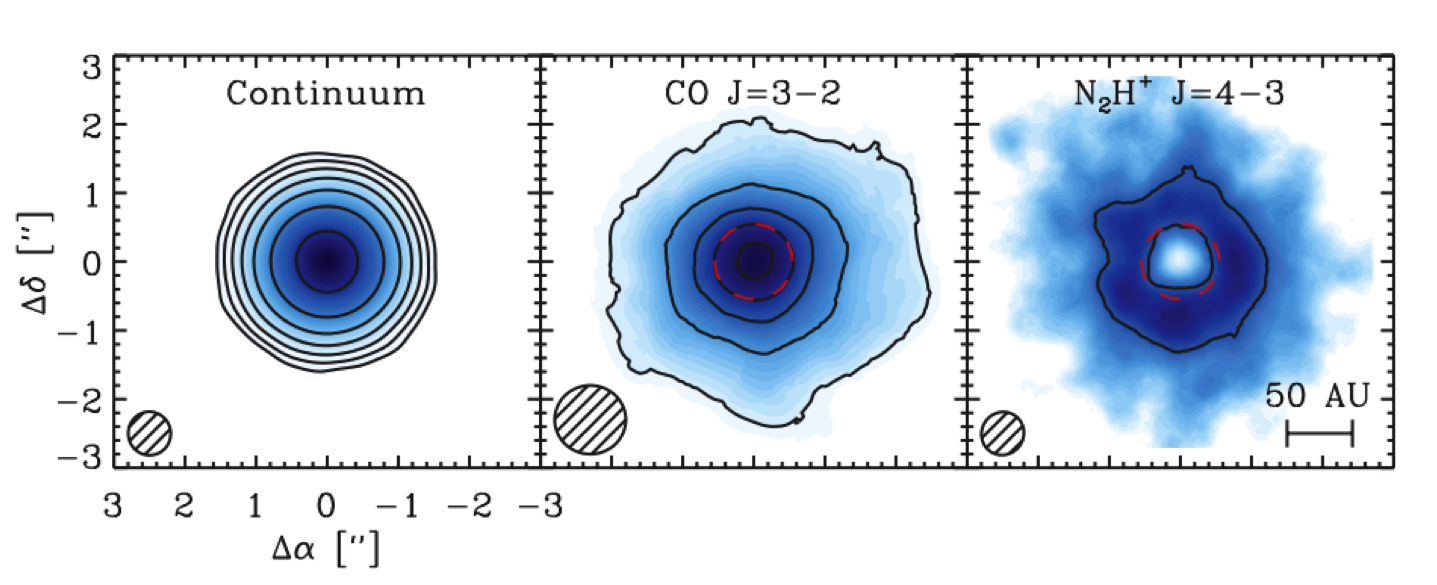
\includegraphics[width=0.8\textwidth]{figures/CO.png}
%\vspace{-0.5in}
\caption{ALMA detection of the CO snowline in TW Hya at 30 AU. Reprinted by permission from Karin \"Oberg.}
\label{fig:qi13}
\end{figure}

%\begin{figure}[t!]
%\centering
%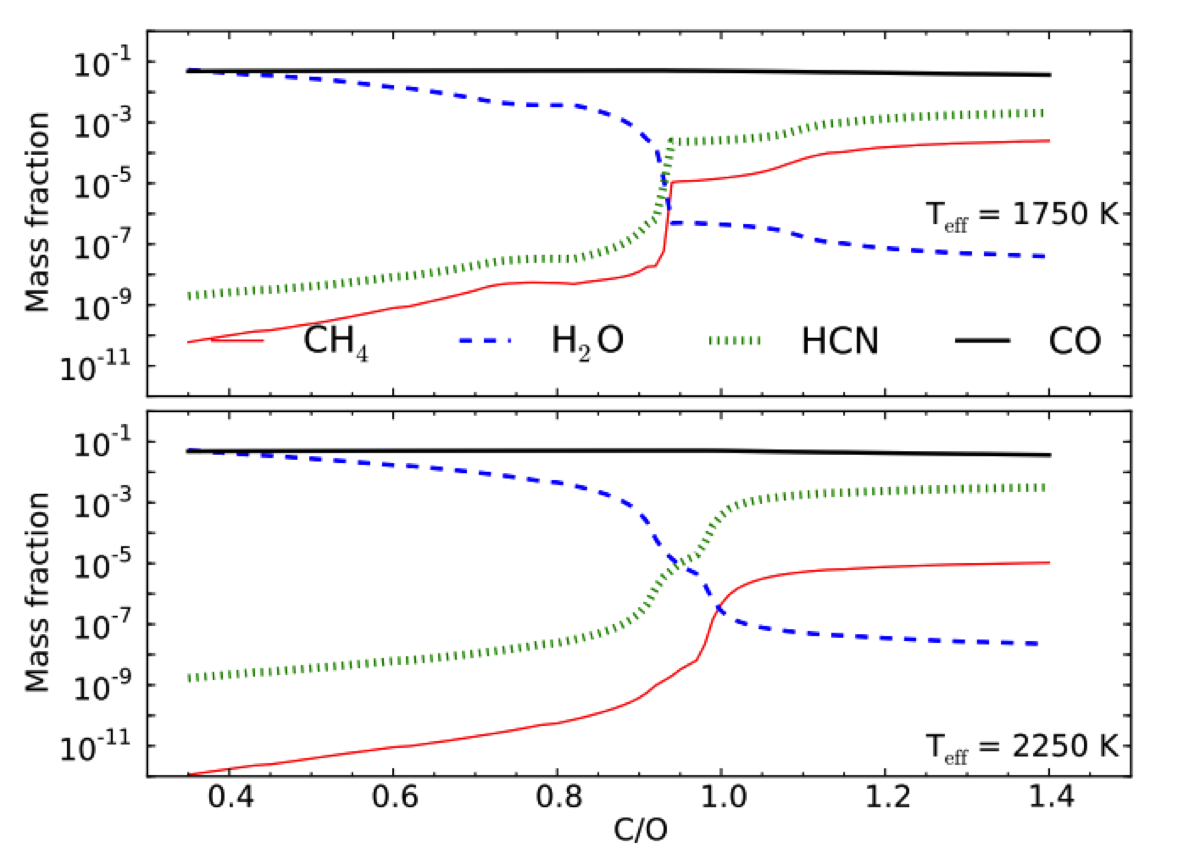
\includegraphics[width=0.8\textwidth]{figures/molliere.png}
%%\vspace{-0.5in}
%\caption{Theoretical model of an exoplanet atmosphere showing that small variations in the C/O ratio produce very large variations in the abundance of other volatiles. From \citet{molliere15}.}
%\label{fig:molliere}
%\end{figure}

%\subsubsection{C/O Ratios in Disks}

One important effect of the existence of snowlines is that disks are expected to contain different amounts of volatiles in gas and in dust at different locations. As the main carbon and oxygen carriers, i.e. H$_2$O, CO$_2$ and CO, are amongst the most abundant volatiles in comets and protostellar cores (\citealt{rodgers02}, \citealt{mumma11}, \citealt{henning13}), variations in the carbon-to-oxygen (C/O) ratio in gas and dust throughout a disk are particularly important. This issue was first addressed by \citet{oberg11}. Figure \ref{fig:oberg} shows the C/O ratio in gas and dust as a function of semimajor axis, assuming protostellar abundances for the volatiles. The C/O ratio in gas is enhanced compared to the stellar value, particularly between the CO$_2$ and CO snowlines where it reaches unity. The pioneering work of \citet{oberg11} inspired Chapter 4 of this thesis. \citet{oberg11} consider a static disk, and thus do not account for dynamical processes such as redistribution of solids due to radial drift, the radial movement of the nebular gas, and accretion heating. We thus expand this model by considering the processes outlined above and their effect on snowline locations. In particular, we focus on how radial drift of solids and viscous gas accretion onto the central star affect the H$_2$O, CO$_2$ and CO snowline locations for particles of different sizes. We find that drift and accretion heating alone may move the snowlines inward by factors of $\sim$2 compared to a static disk, thus substantially changing the disk regions with enhanced gas-phase C/O ratios. %, which has direct consequences for planet formation. 

\begin{figure}[h]
\centering
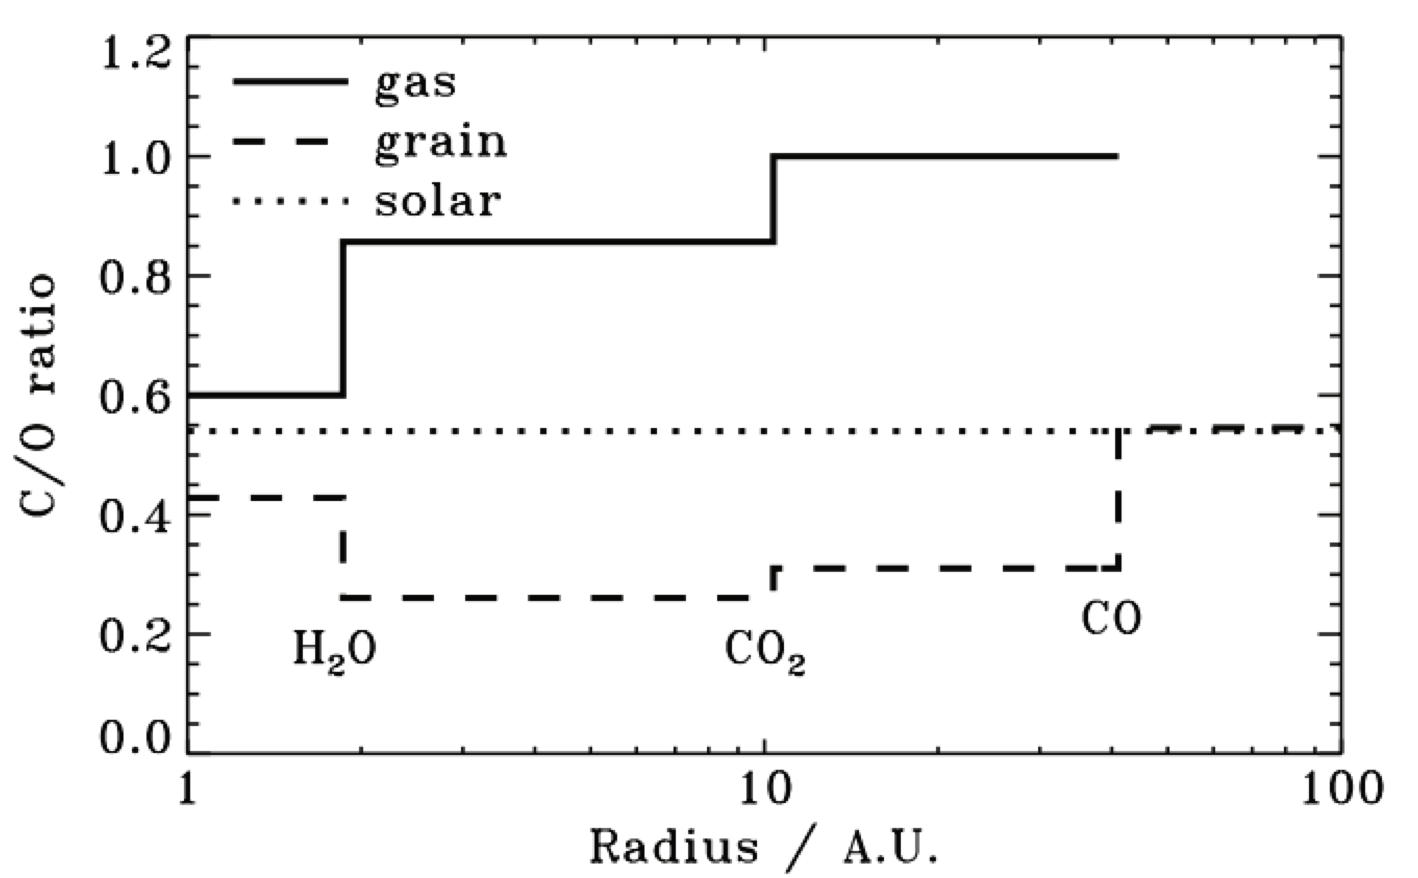
\includegraphics[width=0.8\textwidth]{figures/oberg11.png}
%\vspace{-0.5in}
\caption{The C/O ratio in gas (solid line) and dust (dashed line) as a function of semimajor axis in a static disk. The dotted line shows the stellar value of 0.54. Gas-phase C/O ratios of order unity can be achieved in the outer disk. Reprinted by permission from Karin \"Oberg. }
\label{fig:oberg}
\end{figure}



%\subsubsection{The Importance of Nitrogen}

As we show above, the C/O ratio is highly important to study, but it only provides us with one piece of the puzzle that is constraining planet formation origins based on their compositions. In order to improve our theoretical models, we thus need to look at other molecules and volatile compounds. The first that comes to mind is nitrogen, as it highly abundant in the Solar System \citep{lodders03}, and primarily believed to exist as N$_2$ (e.g., \citealt{owen01}). Molecular nitrogen cannot be detected directly. However, an inventory of nitrogen cometary abundances shows that NH$_3$ is the most abundant observed nitrogen carrier, and yet its concentration is only a small fraction of the total nitrogen abundance, which leaves N$_2$ as the main nitrogen bearing species. In the context of planet compositions, N$_2$ is important due to its high volatility. The gas phase
nitrogen-to-oxygen (N/O) ratio in the outer disk may thus be even more enhanced than the C/O ratio. We calculate the N/O ratio in gas and dust in Chapter 5, and confirm that it is indeed highly enhanced compared to the stellar value throughout most of the disk.

%We note that this differential volatile condensation effect has already been used to explain potential claims hat some planets, such as WASP-12 b, have a superstellar C/O ratio \citep{madhu11}. While this particular detection has since been unequivocally refuted (e.g., \citealt{kreidberg15}), the advent of JWST in the near future will provide us with a significantly larger sample of atmospheric spectra which may be used to constrain C/O ratios in other giant planet atmospheres. 
%
%
%
%While there are several volatiles in disks that can be further investigated, one important signature of atmospheric chemistry is the carbon-to-oxygen (C/O) ratio. This is demonstrated in Figure \ref{fig:molliere}, which shows a theoretical model of an exoplanet atmosphere: variations in the C/O ratio by factors of $\sim$3 change the abundance of other volatiles, such as H$_2$O and CH$_4$ by several orders of magnitude. From the observational perspective, an exciting potential discovery was that some planets, such as WASP-12 b, have a superstellar C/O ratio \citep{madhu11}. While this particular detection has since been unequivocally refuted (e.g., \citealt{kreidberg15}), the advent of JWST in the near future will provide us with a significantly larger sample of atmospheric spectra which may be used to constrain C/O ratios in other giant planet atmospheres. The possibility of a superstellar C/O ratio in a disk or planet atmosphere is also intriguing from a theoretical standpoint. One likely explanation is that the main carbon and oxygen carriers, i.e. H$_2$O, CO$_2$ and CO, have different condensation temperatures. This will result in variations in the abundance of the volatiles in gas and solid form between their respective snowlines, which will subsequently change the C/O ratio at different disk radii. This idea was first postulated by   



\subsection{Ice Morphology}


The snowline locations of volatiles, including carbon, oxygen and nitrogen carriers, are highly dependent on the morphology of the icy particles. These can either form on a dust mantle as pure ices, or have a layered structure with the more volatile species closer to the outer layers (e.g., \citealt{pontoppidan03}). As H$_2$O is the least volatile species with high abundance in disks, one can typically expect the more volatile molecules to form on a water substrate (but see \citealt{bisschop06} for other scenarios). The ice environment in which the molecules reside, i.e. pure or water dominated ices, will determine their binding energies. This, in turn, will change the temperatures at which the ices desorb, and thus their snowline locations. This effect is particularly important in the case of CO and N$_2$, since their volatility is significantly higher than that of other carbon and nitrogen carriers, such as CO$_2$ or NH$_3$. Laboratory experiments \citet{fayolle16} have determined new values for the CO and N$_2$ binding energies, both as pure ices and water dominated. Figure \ref{fig:fayolle} shows the results of a temperature programmed desorption (TPD) experiment for the CO and N$_2$ desorption rate as a function of temperature, in water dominated and pure ice environments. The peak of the desorption curves shifts considerably between the different binding environments. This translates into a difference in binding energies by up to a factor of two between pure and water dominated CO or N$_2$. We show in Chapter 5 that this large difference in binding energies changes the CO and N$_2$ snowline locations by factors of 3-4 spending on the ice environment. By taking into account also the effect of disk dynamics, we find that the CO and N$_2$ snowlines may span several tens of AU. This uncertainty in snowline locations suggests yet again that more observations are needed to constrain disk volatile compositions at different locations. %, and thus trace the origins of gas giants based on their atmospheric compositions.  

\begin{figure}[t!]
\centering
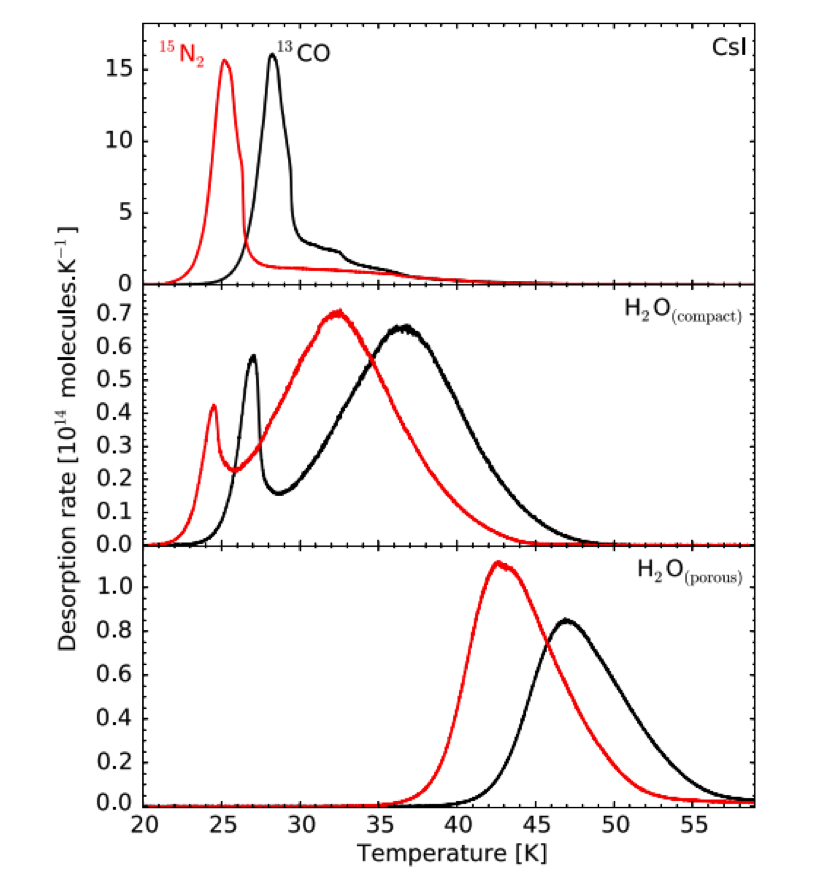
\includegraphics[width=0.8\textwidth]{figures/fayolle.png}
%\vspace{-0.5in}
\caption{Desorption rate as a function of temperature in a TPD experiment, for CO and N$_2$ as pure ices (top panel), on a compact H$_2$O substrate (middle panel), and on porous H$_2$O substrate (bottom panel). The peaks in the desorption curves are at substantially higher temperatures for the water dominated ices. Reprinted by permission from Karin \"Oberg.}
\label{fig:fayolle}
\end{figure}

\subsection{Consequences for the C/N/O Ratio in Planetary Atmospheres}

Variations in the C/O ratio in gas and dust due to different volatile condensation temperatures have also been investigated in exoplanet atmospheres, both from a theoretical and observational standpoint. \citet{molliere15} show that varying the C/O ratio in a gas giant envelope by factors of $\sim$3 changes the abundance of other volatiles, such as H$_2$O and CH$_4$, by several orders of magnitude. From the observational perspective, an exciting potential discovery was that some planets, such as WASP-12 b, have a superstellar C/O ratio \citep{madhu11}. While this particular detection has since been unequivocally refuted (e.g., \citealt{kreidberg15}), the advent of JWST in the near future will provide us with a significantly larger sample of atmospheric spectra which may be used to constrain C/O ratios in other giant planet atmospheres. 

While observational constraints for the N/O ratio in planetary atmospheres do not currently exist, the high gas-phase N/O ratio enhancement at most disk radii suggests that giant planets that form at wide separations should have an excess of nitrogen in their atmospheres, which could be used to trace their formation origin. Theoretical and observational knowledge of both C/O and N/O ratios could further help back-track the planet formation location based on planet composition. 



\section{The Core Accretion Mechanism and Its Challenges}

Gas giants are widely believed to form through core accretion (e.g., \citealt{pollack96}), a theory in which
solid protoplanetary cores grow large enough to accumulate a massive atmosphere. In this
model, planetesimals in a disk grow larger through collisions, eventually forming a planetary
embryo, which continues to grow by attracting planetesimals in its neighborhood. Once an
embryo becomes large enough so that its escape velocity exceeds the thermal velocity of the
nebular gas in its vicinity, it starts accumulating a gaseous envelope. From this point on, the
accretion of gas is regulated by the pressure support within the envelope --- the amount of
gas a core can accumulate is limited by the atmosphere's ability to radiate away the energy
due to the incoming planetesimals, as well as by envelope contraction.

Protoplanetary disks dissipate on relatively short timescales of a few Myr. This implies that cores must grow fast in order to become large enough to attract massive atmospheres, and thus they need high planetesimal accretion rates. Studies that consider such high and constant rates (e.g., \citealt{stevenson82}, \citealt{boden86}, \citealt{wuchterl93}, \citealt{rafikov06}) find that the envelope accumulating around the planet is in steady state at all times, since all the energy due to the incoming planetesimals is radiated away by the atmosphere. It follows that the core and envelope grow simultaneously, and the mass of the atmosphere is a function of the core mass. Once the core and atmosphere have attained comparable masses, a rapid phase of runaway gas accretion starts and the gas giant can form. In this steady state scenario, there is therefore a uniquely determined core mass at which runaway accretion commences, called the critical core mass $M_{\rm crit}$. High planetesimal accretion rates cause the core to grow quickly, but this poses an additional challenge: fast accretion heats up the core's atmosphere, increases pressure support and inhibits the ability of the envelope to cool and contract, thus eventually increasing $M_{\rm crit}$. This is particularly challenging in the outer disk, where long dynamical times prevent large cores from forming before disk dissipation. \citet{rafikov11} shows that core accretion cannot operate beyond 40-50 AU at the accretion rates required to form the core and the atmosphere on the same timescale. 

%\begin{figure}[t!]
%\centering
%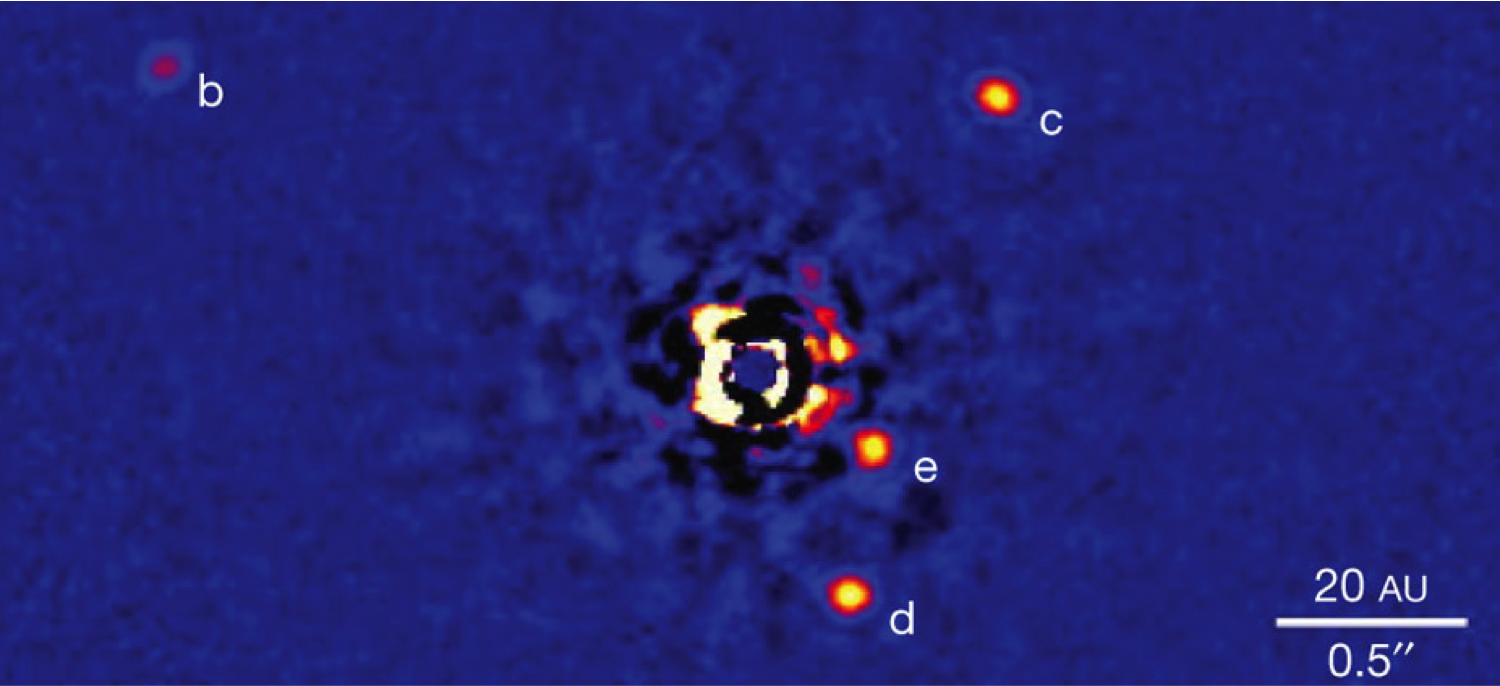
\includegraphics[width=0.8\textwidth]{figures/HR8799.png}
%%\vspace{-0.5in}
%\caption{The directly imaged HR 8799 system. Planets are located at 14.5 AU, 24 AU, 38 AU and 68 AU. From \citet{marois10}. }
%\label{fig:HR8799}
%\end{figure}

All this seems to indicate that core accretion cannot work in the outer disk. This poses an intriguing question: could wide-separation gas giants, such as the HR 8799 system, have formed through core accretion? We can start answering this question by noting that planetesimal accretion does not need to be constant with time at a given location in the disk, which has been shown to be a viable scenario (e.g., \citealt{ikoma00}, \citealt{pollack96}). Figure 1 from \citet{pollack96} shows an example of this scenario. At early times, the core is in a high planetesimal accretion rate regime and grows fast, but the atmosphere remains small in comparison. As the planet depletes its feeding zone of solids, planetesimal accretion is reduced. From this point on, the core no longer grows significantly, and thus the energy due to planetesimals can no longer balance radiative losses by the atmosphere; now the envelope accumulates gas while undergoing Kelvin-Helmholtz contraction, until its mass approximately exceeds the core mass and runaway gas accretion begins. Since now the envelope grows with time, there is no longer a uniquely determined $M_{\rm crit}$ --- in this scenario, the critical core mass is that of a core than can accrete an atmosphere with a mass equal to its own on a timescale equal to the disk lifetime. 

%\begin{figure}[t!]
%\centering
%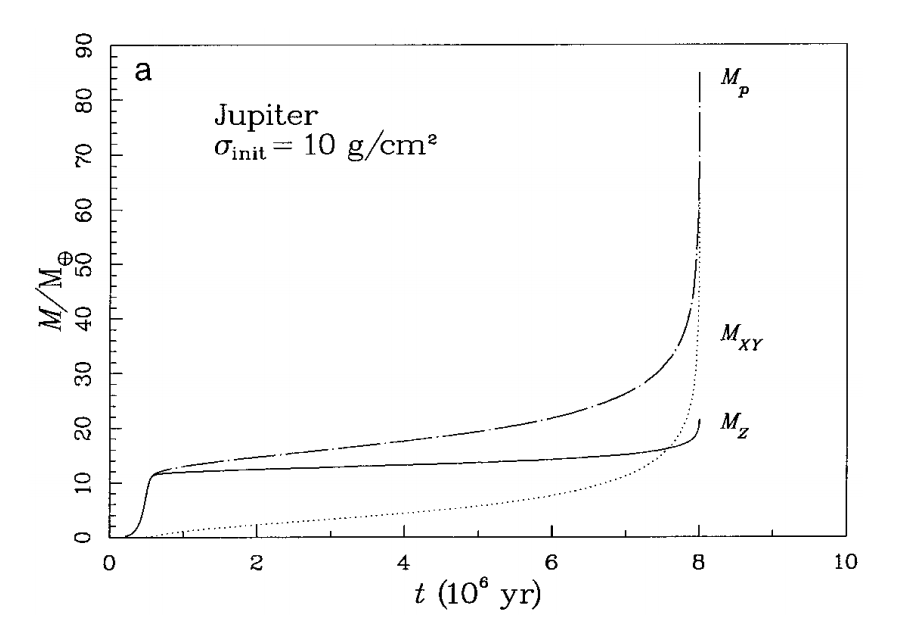
\includegraphics[width=0.8\textwidth]{figures/pollack.png}
%%\vspace{-0.5in}
%\caption{The evolution of a nascent planet's core (denoted with the subscript Z), atmosphere (denoted with the subscript XY), and total mass (denoted with the subscript p) as a function of time, for a planet forming at 5.2 AU through core accretion. The plot depicts the three phases of the planet's evolution: (1) core growth while atmosphere remains small (until $\sim1.2$ Myr), (2) atmospheric growth while core growth is practically stalled (until $\sim$7 Myr), and (3) runaway gas accretion.}
%\label{fig:pollack}
%\end{figure}

Such studies potentially provide a viable solution to the core accretion challenge at wide separations, but they are primarily focused on explaining the formation of Jupiter at 5.2 AU and thus do not explore a larger radii parameter space. Moreover, in order to truly understand whether core accretion can indeed work at stellocentric distances significantly larger than that of Jupiter, a more interesting question can be asked: what is the lowest possible core mass required to form a gas giant before disk dissipation? This minimum core mass is determined when planetesimal accretion has fully stopped, since additional accretion would actually increase this core mass (see above). Moreover, how does this minimum core mass depend on disk location, the properties of the nebular gas, and the opacity of the dust grains? We provide an answer to these questions in Chapters 2 and 3, where we find that the minimum core mass for giant planet formation is lower than the one typically quoted, 10 $M_{\oplus}$ (\citealt{stevenson82}, \citealt{rafikov06}), and may be as low as 1 $M_{\oplus}$. Our study thus reopens the case for in situ formation of wide-separation gas giants through core accretion.   


   

%\subsection{The Role of Disk Location in Setting the Minimum Core Mass for Giant Planet formation}
%
%\begin{itemize}
%
%\item Gas giants are largely believed to form through core accretion (insert core accretion sketch from various talks). This process is particularly challenging in the outer disk due to long dynamical timescales. At the same time, wide separation gas giants have been discovered (HR 8799 plot). This poses an intriguing question: how do these planets form: I answer this question in the first part of my thesis; specifically I calculate the minimum Mcrit, which applies when cores no longer accrete solids. Standard core accretion studies are not built to properly explore this Mcrit. Here explain standard core accretion studies in more detail and insert e.g. one of the Mass vs time figures from Pollack et al. 1996. Explain how our study is different. Finalize by saying that the studies I performed clearly challenge previous claims that  core accretion cannot operate at wide separations, thus reopening the case for in-situ formation of wide separation gas giants.
%
%\end{itemize}
%
%\subsection{The Role of Disk Dynamics and Morphology in Setting Snowline locations and C/N/O Ratios}
%
%\begin{itemize}
%
%\item Disk Composition Regulates Planet Composition. It is thus essential to (1) predict what kinds of planet compositions result from planet location in different parts of the disk, and (2) conversely, bacl-track planet formation location based on planet composition.
%
%\item Disks are complex. Show figure from Henning and Semenov with all processes that occur in disks and discuss which ones I tackle in the thesis.
%
%\item However, we do know some things about disks. Volatile molecules have detected in disks (show figure with Spitzer IR spectrum of AA Tauri). Snowlines have also been detected (show CO snowline plot from Qi+13).
%
%\item One important signature of atmospheric chemistry is the C/O ratio (explain why and show plot from Molliere+15 which shows the effect of varying C/O ratio on the abundance of other volatiles). Discuss claims that super stellar C/O ratios have been detected (show Wasp 12-b spectrum from Madhusudhan), but have since been refuted. Explain that this poses an intriguing question from a theoretical standpoint. Mention idea proposed by Oberg+11 (show plot). Discuss that disk dynamics have an important role, which is partly what we tackle in this part of the thesis.
%
%\item There are other important volatiles besides H2O, CO2 and CO. Discuss the importance of N2 and show plot with abundances in comets that show that NH3 is the main carrier based on observations, but it doesn't account for all the nitrogen in the solar system. 
%
%\item Ice morphology is important. Discuss why. Discuss how binding energies depend on the ice environment and show plot from Edit's paper. 
%
%\item It follows that we have to take into account additional volatiles, abundances and ice morphologies besides disk dynamics to see their effect on snowline locations and the C/N/O ratios. We tackle this in Chaper xx.
%
%\item We demonstrate in this part to the thesis that C/N/O ratios may be used to track a planet's formation origin, when combined with observations, but that more observations are needed.
%
%\end{itemize}

\section{The Disk-Planet Connection}

Our work in the two main parts of this thesis confirms that there is indeed a tight link between disks and planets. Our study on core accretion shows that the core mass required to form a gas giant is highly dependent on the disk properties and composition, while our chapters on snowline locations and C/N/O ratios also demonstrate that the disk structure and chemical composition has direct effects on the volatile composition of giant planets atmospheres. This thesis thus sets the stage to uncovering the role of disk volatile composition, dynamics and chemistry in shaping the compositions of nascent giant planets. 

